\subsubsection*{Problem definition}

The non-linear Langmuir isotherm is used to describe sorption processes that are restricted by a maximum concentration of sorbed molecules. In this example, the transport process by including the Langmuir isotherm is calculated in the same way as in the precedent examples for mass transport. As there exists no opportunity to calculate analytically the solute transport with non-linear sorption, the results of the simulation have to be compared with solutions of the transport equation with linear sorption in order to evaluate the simulation results.

\textsl{Assumptions}

\begin{tabbing}
Component: \= non-linear sorption with maximum concentration (Langmuir isotherm)\\
\> no decay \\
Aquifer: \> homogeneous, saturated, stationary flow \\
\end{tabbing}

\subsubsection*{Model set-up of the 1~D numerical model}

See chapter \ref{sec:decay}

The soil parameters are the same as listed in table \ref{tab51}(except decay). In order to create a Langmuir equation which has almost the same linear characteristic as the Henry equation, the Langmuir sorption coefficients, K$_1$, were varied in the same way as the Henry coefficients (K$_D$ values in table \ref{tab52}) for the different simulation runs. The K$_2$ coefficients stand for the affinity between solid and sorbed solute. Thus, the K$_2$ value can not be set equal to 0, because this would cause a transport without any sorption. When K$_2$ equals 1, there is no effect on the binding affinity. Therefore, the coefficient K$_2$ was set constant with a value of 1 in order to approximate the linear characteristic of the Henry equation (\ref{eq58}).

\subsubsection*{Evaluation method}
The dependence of sorbed molecules on the amount of molecules in dilution is given by equation \ref{eq510}. The concentration distribution at a special point in time and over a given distance cannot be calculated analytically by equation \ref{eq53} when a non-linear sorption process is assumed. Therefore, the simulation results are compared with the results for the mass transport by using the linear Henry isotherm. The non-linear Langmuir isotherm was forced to be almost linear in the way as described above. Now the results of the transport by using the Langmuir isotherm can be compared with the results that were obtained by the transport simulation with the linear Henry isotherm.

\subsubsection*{Results}

In figure \ref{fig56} the concentration distributions over the whole model length by using the linear Henry isotherm and the non-linear Langmuir isotherm are depicted. Obviously, the results for each specified distribution constant are almost equal. This result is correct, because it was provoked by the choice of the sorption coefficients.

\begin{figure}[htbp]
\centering
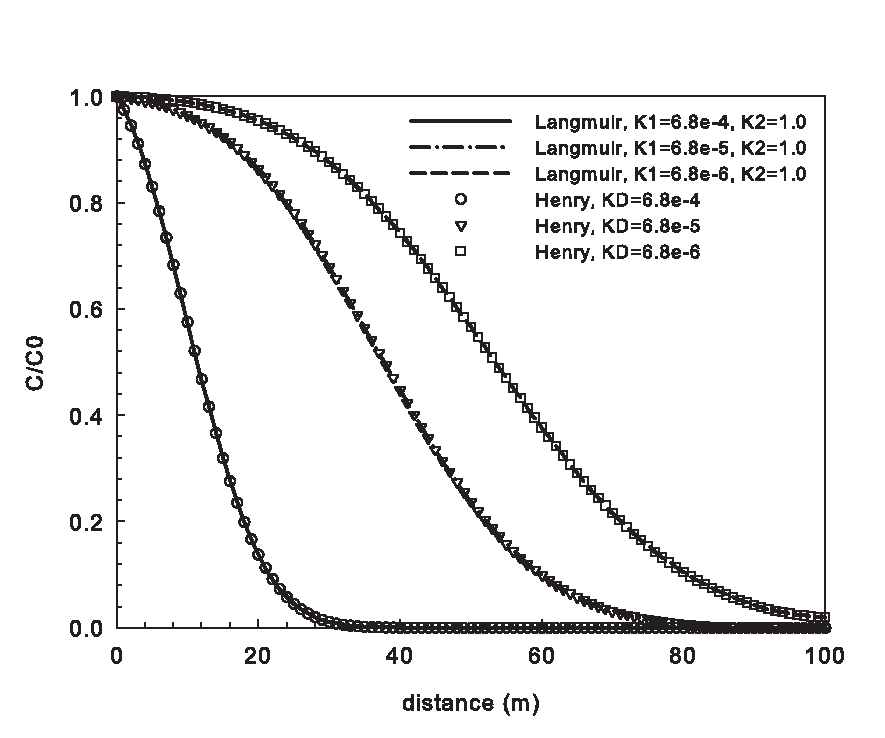
\includegraphics[width=0.8\textwidth]{C/figures/fig56.EPS}
\caption{Concentration distribution after 100~d (Langmuir compared to Henry sorption)}
\label{fig56}
\end{figure}

In order to show that the results by the use of the Langmuir isotherm are actually different to those by using the Henry isotherm, the K$_2$ values were changed to a value of 0.8, so that the Langmuir isotherm got a real non-linear gradient. As the results show (fig. \ref{fig57}), the differences between the concentration distributions are evident.

\begin{figure}[htbp]
\centering
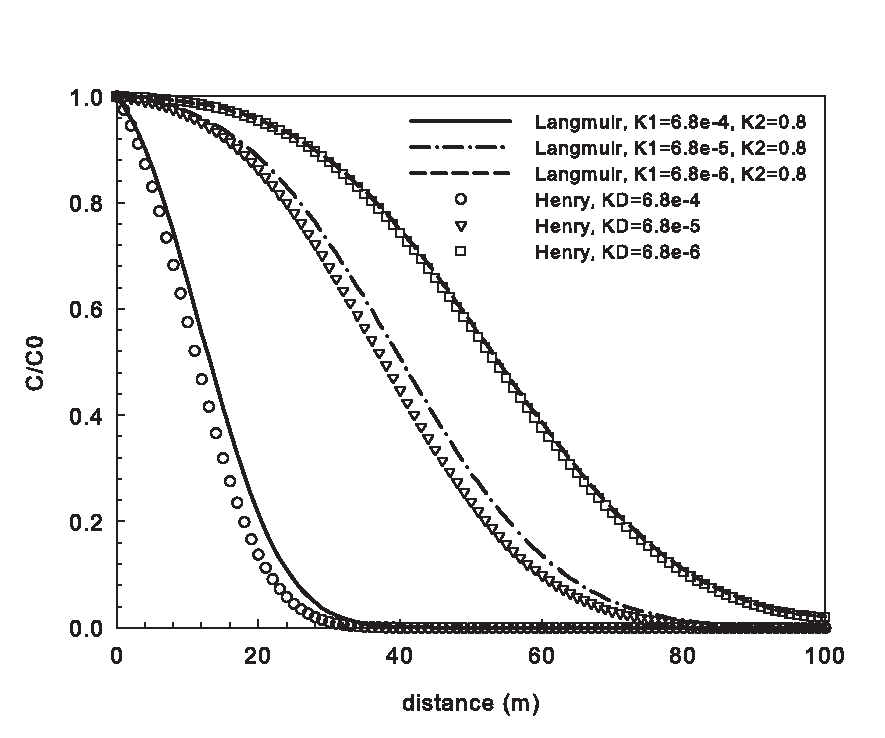
\includegraphics[width=0.8\textwidth]{C/figures/fig57.EPS}
\caption{Different concentration distributions after 100~d (Langmuir compared to Henry sorption)}
\label{fig57}
\end{figure}

\begin{tabular}{|l|l|l|}
\hline
Benchmark & Problem type	& Path in benchmark deposit \\
\hline	
hc\_sorp\_langmuir\_1D	& HC	& benchmarks $\backslash$HC$\backslash$Sorption$\backslash$Langmuir \\
\hline	
\end{tabular}
